%!TEX TS-program = xelatex
%!TEX encoding = UTF-8 Unicode

\documentclass[12pt]{extarticle}
% extarticle is like article but can handle 8pt, 9pt, 10pt, 11pt, 12pt, 14pt, 17pt, and 20pt text

\def \ititle {Origins of Mind}
 
\def \isubtitle {Lecture 08}
 
\def \iauthor {Stephen A. Butterfill}
\def \iemail{s.butterfill@warwick.ac.uk}
\date{}

%for strikethrough
\usepackage[normalem]{ulem}

\input{$HOME/Documents/submissions/preamble_steve_handout}

%\bibpunct{}{}{,}{s}{}{,}  %use superscript TICS style bib
%remove hanging indent for TICS style bib
%TODO doesnt work
\setlength{\bibhang}{0em}
%\setlength{\bibsep}{0.5em}


%itemize bullet should be dash
\renewcommand{\labelitemi}{$-$}

\begin{document}

%\raggedcolumns

\begin{multicols*}{3}

\setlength\footnotesep{1em}


\bibliographystyle{newapa} %apalike

%\maketitle
%\tableofcontents




%--------------- 
%--- start paste


\def \ititle {Logic I}
 
\def \isubtitle {Lecture 01}
 
\begin{center}
 
{\Large
 
\textbf{\ititle}: \isubtitle
 
}
 
 
 
\iemail %
 
\end{center}
 
Readings refer to sections of the course textbook, \emph{Language, Proof and Logic}.
 
 
 
\section{The Pigs of Logic}
 
\emph{Reading:} §1.1, §1.2, §2.1
 
\textbf{Argument 1:} \begin{quote} Either it went up the left fork or it went up the right fork.

It didn’t go up the left fork.

therefore:

It went up the right fork. \end{quote}

\textbf{Argument 2:} \begin{quote} Either it went up the left fork or it went up the right fork.

The left fork is unsuitable for pigs.

therefore:

It went up the right fork. \end{quote}

 
\begin{minipage}{\columnwidth}
 
\textbf{FOL version of Argument 1:}
 
\begin{center}
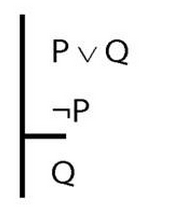
\includegraphics[scale=0.3]{img/argument1_fol.png}
\end{center}
\end{minipage}
 
 
 
\section{Why Logic?}
 
‘Logic pervades the world: the limits of the world are also its limits.’
(Wittgenstein, Tractatus 5.61)
 
‘If a card has a vowel on one side, then it has an even number on the other side.’
(Waison \& Johnson-Laird 1972)
 
\begin{center}

\includegraphics[scale=0.3]{img/waison_fig.png}
\end{center}
 
 
\section{Quick Intro to Logiya (‘FOL’)}
 
\emph{Reading:} §1.1, §1.2, §1.3
 
\begin{center}
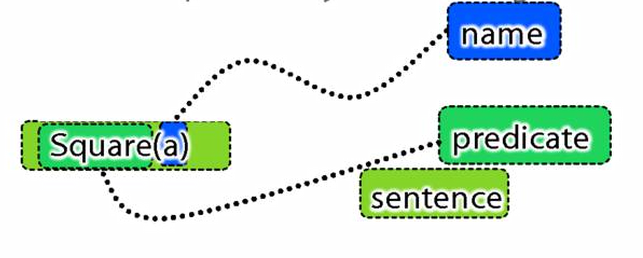
\includegraphics[scale=0.3]{img/name_predicate_sentence.png}
\end{center}
A formal langauge enables us to avoid ambiguity, e.g.:
 
\begin{quote}
 
This is a hospital where doctors are trained.
 
\end{quote}
 
A formal langauge also enables us to some avoid appearance--reality problems:
 
\begin{quote}
 
Many more people have been to Paris than I have.
 
\end{quote}
 
 
 
\section{Logically Valid Arguments}
 
\emph{Reading:} §2.1
 
An argument is \emph{logically valid} just if there’s no possible situation in which the premises are true and the conclusion false
 
 
 
\section{Identity}
 
\emph{Reading:} §2.2
 
Principle: If b=c then whatever is true of b is also true of c.
 
Principle: a=a is never false
 
\begin{center}
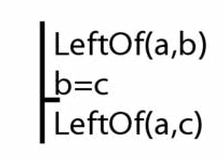
\includegraphics[scale=0.3]{img/arg_identity.png}
\end{center}
 
 
\section{Counterexamples}
 
\emph{Reading:} §2.5
 
A \emph{counterexample} to an argument is a possible situation in which its premises are T and its conclusion F.
 
There are no counterexamples to a logically valid argument.
 
If an argument is not valid, then there is a counterexample to it.
 
To show that an argument is not logically valid, we specify a counterexample to it.
 
 
 
\section{Soundness}
 
An argument is \emph{sound} just if it is logically valid and its premises are true
 
Whether a sentence is true may change as the world changes.
 
The same applies to whether an argument is sound.
 
Whether an argument is logically valid not does change as the world changes.

\vfill

\begin{minipage}{\columnwidth}
\section{Exercises}
These exercises will be discussed in seminars the week after this lecture.
The numbers below refer to the numbered exercises in the course textbook, e.g. `1.1' refers to exercise 1.1. on page 39 of the second edition of \emph{Language, Proof and Logic}.
 
\begin{quote}
1.1--1.5
 
*1.6
 
1.8--1.10
 
2.3, 2.4
 
\end{quote}
\end{minipage}
 

%--- end paste
%--------------- 
 
\footnotesize 
\bibliography{$HOME/endnote/phd_biblio}

\end{multicols*}

\end{document}